%%%%%%%% ICML 2019 EXAMPLE LATEX SUBMISSION FILE %%%%%%%%%%%%%%%%%

\documentclass{article}

% Recommended, but optional, packages for figures and better typesetting:
\usepackage{microtype}
\usepackage{graphicx}
\usepackage{subfig}
\usepackage{booktabs} % for professional tables

% hyperref makes hyperlinks in the resulting PDF.
% If your build breaks (sometimes temporarily if a hyperlink spans a page)
% please comment out the following usepackage line and replace
% \usepackage{icml2019} with \usepackage[nohyperref]{icml2019} above.
\usepackage{hyperref}

% Attempt to make hyperref and algorithmic work together better:
\newcommand{\theHalgorithm}{\arabic{algorithm}}

% Use the following line for the initial blind version submitted for review:
\usepackage{icml2019}

% If accepted, instead use the following line for the camera-ready submission:
%\usepackage[accepted]{icml2019}

% The \icmltitle you define below is probably too long as a header.
% Therefore, a short form for the running title is supplied here:
\icmltitlerunning{System Identification through Expression Optimization}


%%%%%%%% this region contains all the stuff Anthony Added %%%%
\usepackage{vector}
\usepackage{amsfonts}
\usepackage{amsmath}
\usepackage{cleveref}
\newcommand{\todo}[1]{\textbf{[[#1]]}}
\renewcommand{\vec}[1]{\vect{#1}}
\newcommand{\mat}[1]{\vect{#1}}
%%%%%%%%%%%%%%%%%%%%%%%%%%%%%%%%%%%%%%%%%%%%%%%%%%%%%%%%%%

\begin{document}

\twocolumn[
\icmltitle{System Identification through Expression Optimization}

% It is OKAY to include author information, even for blind
% submissions: the style file will automatically remove it for you
% unless you've provided the [accepted] option to the icml2019
% package.

% List of affiliations: The first argument should be a (short)
% identifier you will use later to specify author affiliations
% Academic affiliations should list Department, University, City, Region, Country
% Industry affiliations should list Company, City, Region, Country

% You can specify symbols, otherwise they are numbered in order.
% Ideally, you should not use this facility. Affiliations will be numbered
% in order of appearance and this is the preferred way.
\icmlsetsymbol{equal}{*}

\begin{icmlauthorlist}
\icmlauthor{Anthony Corso}{stanford}
\icmlauthor{Mykel Kochenderfer}{stanford}
\end{icmlauthorlist}

\icmlaffiliation{stanford}{Department of Aeronautics and Astronautics, Stanford University, Stanford, California, USA}

\icmlcorrespondingauthor{Anthony Corso}{acorso@stanford.edu}
\icmlcorrespondingauthor{Mykel Kochenderfer}{mykel@stanford.edu}

% You may provide any keywords that you
% find helpful for describing your paper; these are used to populate
% the "keywords" metadata in the PDF but will not be shown in the document
\icmlkeywords{Machine Learning, ICML}

\vskip 0.3in
]

% this must go after the closing bracket ] following \twocolumn[ ...

% This command actually creates the footnote in the first column
% listing the affiliations and the copyright notice.
% The command takes one argument, which is text to display at the start of the footnote.
% The \icmlEqualContribution command is standard text for equal contribution.
% Remove it (just {}) if you do not need this facility.

%\printAffiliationsAndNotice{}  % leave blank if no need to mention equal contribution
\printAffiliationsAndNotice{\icmlEqualContribution} % otherwise use the standard text.

\begin{abstract}
Many successful machine learning algorithms find patterns in data using complex and uninterpretable models. This work describes an approach to system identification that requires minimal domain knowledge and discovers governing equations that are parsimonious, generalizable, and interpretable. This approach is enabled by techniques in expression optimization that allow for the automated discovery of mathematical expressions from a combinatorially large set of possibilities. Using simulated data, our approach correctly identifies both linear and nonlinear partial differential equations including the Navier-Stokes equations, as well as discovers exact and approximate Koopman eigenfunctions for nonlinear dynamical systems. 
\end{abstract}

\section{Introduction}
\label{introduction}

Over the past several decades, machine learning has made significant strides in learning patterns from large amounts of data. Although accurate, these systems often produce models that are not interpretable by the human researchers who use them. They often do not report a causal explanation for their predictions and can generalize poorly when the task is altered. Constructing intrepretable and generalizable models will allow researchers to better understand and control important physical systems such as complex fluid flows for more efficient energy generation and transportation.

% [TAKE 2: Over the past several decades, machine learning has made great strides in learning patterns from large amounts of data. Being able to detect patterns from data will be instrumental in allowing scientists to better understand patterns within the earth's climate or fluid flow to design more efficient energy generation and transportation. However, many of the current systems are not ideal because they produce results that are not interpretable by the human researchers who create them. The systems do not report an explanation for their prediction (or return a serious of mathematical expressions that can be understood by a domain expert). This means that the results cannot be generalized or applied to similar systems. ]

System identification refers to the process of finding models that are simple and generalize well to similar systems. For maximum interpretability, a system identifier should output models expressed in mathematical terms that are understandable by a domain expert. Examples of interpretable models are partial differential equations (PDEs), ordinary differential equations (ODEs), or explicit functions that transform a nonlinear dynamical system into a linear one. 

It is computationally challenging to find an effective and parsimonious mathematical model from data. Finding such a model requires the generation of a set of possible mathematical descriptions (of which there are uncountably many) and then searching that set for the best subset that describes the data.
 
Current system identification approaches tend to fall into one of three categories: (1) approaches that require little user input but produce results that are difficult to interpret, (2) approaches that produce interpretable output but require significant prior knowledge to use, and (3) approaches that automatically generate mathematical expressions but are limited to finding single, complex expressions.

The first category contains methods like Dynamic Mode Decomposition (DMD) \cite{schmid2010dynamic, kutz2016dynamic}, which projects the dynamics of a system onto the proper orthogonal decomposition (POD) of the state-space. The result is a low-dimensional, linear model of the dynamics, which can be used for prediction and control. However, the POD modes do not describe the dynamical system in a way that connects with domain-specific concepts, making DMD less interpretable by human researchers. Another approach is used by \citet{morton2018deep} where a deep convolutional neural network is used to linearize a high-dimensional nonlinear fluid system. The resulting linearization is contained in a complicated neural network that cannot easily be understood.

The second category includes the method of \citet{brunton2016discovering} known as sparse identification of nonlinear dynamical systems (SINDy), which has been applied to PDEs \cite{rudy2017data} and dynamical systems with limited data \cite{kaiser2018sparse}. SINDy uses sparse regression on a set of features that are provided by the user to determine which are most effective at explaining the data. A similar technique is used in inductive process modeling \cite{bridewell2008inductive, langley2015heuristic}, which is typically applied to ODEs with many state variables. The system of \citet{krizman1995discovering} can generate new feature functions but requires a comprehensive search of all possible features combinations, making it challenging to scale to larger problems. There have also been attempts to linearize nonlinear dynamical systems by explicitly defining a set of basis functions for a nonlinear mapping to linearize a dynamical system \cite{williams2015data, johnson2018class}. These approaches have been largely successful, but they require the user to define the basis functions. 

The third category contains approaches that use expression optimization to produce mathematical relationships that explain data from dynamical systems \cite{hitoshi1995numerical,gray1998nonlinear,rodriequez2004identifying,madar2005genetic}. These methods use genetic programming to evolve an expression tree until a mathematical relationship is discovered that matches the input data. A drawback to these approaches is that they all attempt to find a single explanatory relationship in the data which becomes intractable for systems with many terms and multiple variables. Most dynamical systems have individual additive terms (or processes) that contribute to the dynamics of the system. This structure can be utilized to scale the optimization task to larger problems, as will be demonstrated below. The existing expression optimization methods have not been extended to the challenging domains of PDE identification and system linearization.

This work describes an approach for system identification that produces interpretable models from data with minimal user input and domain knowledge. The user specifies a small set of basic rules from which possible mathematical descriptions can be generated. Then, an optimization technique is applied to make searching such a vast space of possibilities more tractable, seeking the simplest expressions that can explain the supplied data. Our technique combines the ideas of sparse regression with expression optimization to create a hybrid system that has benefits from both areas. Relaxing the requirement to explicitly enumerate possible expressions, allows this new approach to tackle the challenging problem of deriving approximate Koopman eigenfunctions for the linearization of nonlinear systems.

This paper is organized as follows: \cref{systemidentification} describes how governing equations could be derived from data as well as the connection between equation discovery and the approximation of the Koopman operator. \Cref{sieo} details the approach known as system identification through expression optimization (SIEO), and \cref{results} reports the results of SIEO applied to four model systems. Finally, \cref{conclusion} concludes and discusses directions for future investigation. 



\section{System Identification}
\label{systemidentification}

The goal in system identification is to take in data and find a parsimonious description of a dynamical system. This section outlines two goals for system identification: (1) discovery of governing equations expressed as PDEs, and (2) the generation of approximate Koopman eigenfunctions for the linearization of nonlinear systems.

\subsection{Governing Equations}
One approach to understanding a dynamical system is to determine its underlying governing equations. If the system is a spatio-temporal process, then governing equations can be written as PDEs of the form
\begin{equation}
    \frac{\partial \vec{x} (\vec{r},t)}{\partial t} = \theta_1 \vec g_1(\vec{x}(\vec{r},t)) + \ldots + \theta_n \vec g_n(\vec{x}(\vec{r},t))
\end{equation}
where $\vec{r}$ represents the spatial dimensions, $\vec{x}$ contains the state variables, $\vec{g}_i$ are feature functions, and $\theta_i$ are the corresponding coefficients. Given a mapping $\vec{g}_i$, and a state $\vec{x}$, the coefficients of the PDE can be found using a linear model of the form 
\begin{equation}
 \vec{y} = \vec{\theta}^T \tilde{\vec{x}}
 \end{equation}
where $\vec{y} = \partial \vec{x}/ \partial t$ and $\tilde{\vec{x}} = \begin{bmatrix} \vec{g}_1(\vec{x}), \ldots, \vec{g}_n(\vec{x}) \end{bmatrix}^T$. An approximation of $\vec \theta$ can be found by sampling many $\vec{y}$ and $\tilde{\vec{x}}$ points and then performing multiple linear regression. The goal is to find the optimal set of features $\vec{g}_i$ (and corresponding $\theta_i$) for producing the best fit between $\vec{y}$ and $\tilde{\vec{x}}$.

When discovering a governing equation, only the input data is transformed by a nonlinear mapping, while the output data remains unchanged. If a nonlinear mapping were found that could be applied to both the input and output, then it would be possible to convert a nonlinear system into a linear one. This is known as finding the Koopman operator of a system and it is discussed in the next section.

\subsection{Koopman Operators}
Nonlinear dynamical systems are far more challenging to understand and control than their linear counterparts. One promising area of analysis is Koopman theory \cite{korda2018linear} which states that any nonlinear dynamical system can be converted into a linear system under the state-space mapping
\begin{equation}
\vec{x} \mapsto \vec{g}(\vec{x})
\end{equation}
where $\vec{g}(x) = \begin{bmatrix} \vec{g}_1(x), \vec{g}_2(x), \ldots \end{bmatrix}^T$ are the Koopman eigenfunctions. In general, $\vec{g}$ can be infinite-dimensional and is often approximated with a finite-dimensional mapping.

The Koopman operator can take a nonlinear dynamical system of the form
\begin{equation}
\vec{x}^{t+1} = \vec{f}(\vec{x}^t)
\end{equation}
and transform it into the linear system
\begin{equation}
\label{fig:linsys}
\vec{g}(\vec{x})^{t+1} = \mat{K} \vec{g}(\vec{x})^{t}
\end{equation}
Thus, if the the Koopman operator is known, all of the mathematical technologies developed around linear systems can be brought to bear on a nonlinear system. 

If the Koopman eigenfunctions contain the identity function $\vec{g}(\vec{x}) = \vec{x}$ then the Koopman operator is said to be \emph{state-inclusive} and the un-transformed state of the system can be found directly from the linear system (\cref{fig:linsys}), without finding an inverse transformation $\vec{g}^{-1}$.

Given a finite approximation to the Koopman eigenfunctions $\vec{g}(\vec{x}) = \begin{bmatrix} \vec{g}_1(\vec{x}), \ldots, \vec{g}_n \end{bmatrix}^T$, the matrix $\mat{K}$ can be found using a linear model of the form 
\begin{equation}
\vec{y} = \mat{K} \tilde{\vec{x}}
\end{equation} 
where $\vec y = \vec{g}(\vec{x}^{t+1})$ and $\tilde{\vec{x}} = \vec{g}(\vec{x}^t)$. If many points are sampled for $\vec{y}$ and $\tilde{\vec{x}}$ then multiple linear regression can provide the least-squares estimate of $\mat{K}$. The goal for approximating the Koopman operator is to find a finite approximation $\vec{g}(\vec{x})$ that creates the best fit between $\vec{y}$ and $\tilde{\vec{x}}$.

It should now be clear that the problems of equation discovery and approximating the Koopman operator are identical except for the transformation of the output data in the latter case. The next section describes an approach to finding these nonlinear mappings.

\section{System Identification through Expression Optimization (SIEO)}
\label{sieo}
The process of discovering a nonlinear mapping for system identification from data has three steps:
\begin{enumerate}
    \item Define a set of nonlinear functions (referred to as \emph{features}).
    \item Define a loss function to measure the success of a set of features (referred to as a \textit{mapping}).
    \item Search through the possible mappings to find the optimum.
\end{enumerate}
The first and third task each involve searching through a combinatorially large set of possibilities and therefore pose a substantial computational challenge. The first subsection below discusses how the first task can be performed efficiently using a context-free grammar. The second subsection describes two useful loss functions, each for a different system identification task. Finally, the last subsection describes a search technique that combines expression optimization with a greedy heuristic search for finding the optimal mapping. The combination of these techniques comprises the approach we call System Identification through Expression Optimization (SIEO).

\subsection{Context-Free Grammar}

% Motivate the need for a grammar
There are an infinite number of possible mathematical expressions that could be included in a mapping, but researchers do not generally know beforehand which specific expressions will be good candidates. A design goal of SIEO, therefore, is to require minimal prior knowledge from the user while still constraining the possible expressions to be searched.

% Describe what the grammar is
SIEO relies on a domain-specific \textit{grammar}, provided by the user, that gives the rules for generating feature functions \cite{kochenderfer2019algorithms}. A grammar is a set of production rules that govern a language (or a set of expressions). Each rule can either be \textit{non-terminal}, where it relates generic expressions together (e.g. multiplication), or \textit{terminal}, where an expression is concretely defined (e.g. the observed data). Each expression in the language can be represented by a tree of operators, each of which is part of the grammar. Once a grammar is defined, expressions can be sampled from the grammar with varying levels of complexity (as defined by the depth of the expression tree).

% Given an example of a sample from the grammar
For example, the grammar in \cref{fig:advdifgrammar} has rules for differentiation, multiplication, and division. Sampling from a grammar is a process of selecting production rules and then filling in any non-terminal expressions until only terminal expressions remain. For example, in the expression 
\begin{equation}
    u \frac{\partial u}{\partial x }
\end{equation}
the first (non-terminal) production rule chosen is multiplication. Then, on the left side, the terminal expression $u$ was chosen, and on the right side, the non-terminal derivative rule was chosen, followed by the terminal expression $u$. Grammars define a constrained, but still infinite, set of possible expressions. The set can be made finite by specifying a maximum expression depth for a grammar. 

The benefit of this approach is two-fold:
\begin{enumerate}
    \item For the cost of defining a simple grammar, an infinite number of possible expressions (ranging from simple to complex) can be produced.
    \item Researchers can encode into the grammar any information they may have regarding relationships between the input and output data.
\end{enumerate}
As will be demonstrated in later sections, many familiar PDEs have features that come from a very simple grammar (2--3 rules) with a very short depth (2--3). The next subsection describes the loss functions used to compare different mappings.  

\subsection{Choice of Loss Function}
\label{lossfunction}
When attempting to discover a governing equation to explain data, the objective is to find a mapping that is simple (i.e. it has few features) but also describes the output data well. To balance this multi-objective, the negative adjusted $R^2$ value ($-R_{\rm adj}^2$) of the fit can be used for the loss function. The traditional $R^2$ value always increases when new features are added so it makes the algorithm susceptible to overfitting. The adjusted value, however, penalizes the addition of more features using
\begin{equation} 
R_{\rm adj}^2 = R^2 - \alpha (1-  R^2)(n-1)
\end{equation}
where $n$ is the number of features in the mapping. When $n=1$ this expression reduces to the traditional $R^2$ value, but when $n>1$ the difference between $R^2$ and 1 is scaled by the number of parameters. Thus, generally, $\alpha \in [0, \infty)$ should be large when agreement between the input and output (i.e. for synthetic, noise-free data) is expected and should be closer to 0 when near-perfect agreement is not expected (i.e. real world data). The loss function is explicitly defined as 
\begin{equation}
    \ell_R(\theta, \vec{g}) = - R_{\rm adj}^2(\vec{\theta}, \vec{g})
\end{equation}
For the goal of discovering Koopman eigenfunctions, however, parsimony is no longer a consideration so a new loss function is needed. Given a linear system with $n_g$ Koopman eigenfunctions, the loss function associated with the Koopman operator $\mat{K} \vec{g}$ is
\begin{equation} \ell_k(\mat{K} \vec{g}) = \frac{1}{n_g}\lVert \overline{\vec{g}}(\vec{x})^{t+1} - \overline{\mat{K} \vec{g}}(\vec{x})^{t}\rVert _2^2 \end{equation}
where the bar indicates that each feature is normalized to a zero mean and standard deviation of 1. The loss is scaled by $1/n_g$ so the algorithm is not penalized for adding more Koopman eigenfunctions, and instead focuses on closely matching each new state variable when new features are added. This loss function is referred to as the \emph{average normalized sum of squares} loss and should be used when parsimony is not a consideration. The following subsection ties together the use of a grammar and a loss function to explain how expression optimization and heuristic search are used to select features.


\subsection{Feature Selection Algorithms}

One major challenge of system identification is the selection of a mapping from a group of possible features. If there are $N$ possible features, then there are $2^N$ possible subsets from which to choose. It is infeasible to exhaustively search the entire space of combinations for even moderate values of $N$.

Previous approaches have used sparsity-promoting regression techniques such as LASSO \cite{tibshirani1996regression}, but these approaches are brittle when the input data suffers from multicollinearity \cite{rudy2017data}. It was found that the most effective heuristic was a modified form of a greedy search algorithm that combined both forward and backward search. The high-level structure of the algorithm is given in \cref{alg:featureselection}.

The algorithm starts by performing a greedy forward search (\cref{alg:forwardsearch}), where on each iteration a feature is greedily added to the mapping until there is either no further improvement in the loss function or a specified threshold is met. Then, the feature selection algorithm performs a greedy backward search (\cref{alg:backwardsearch}) on the mapping where features are removed if their absence reduces the loss function. This entire process iterates until there is no further improvement of the mapping, at which point it is returned.

The substantial missing piece of this process is how to find the next feature to add to the list. As described previously, a comprehensive search is infeasible, so an expression optimization technique must be used.


\begin{algorithm}[tb]
   \caption{Feature Selection}
   \label{alg:featureselection}
\begin{algorithmic}
   \STATE {\bfseries Input:} Loss function $\ell_f$ \\
   \quad \quad \quad New feature generator $n_f$ \\
   \quad \quad \quad Threshold $t$ \\
   \STATE Initialize $mapping \gets [ \ ]$
   \REPEAT
   \STATE $old\_mapping \gets mapping$
   \STATE $mapping \gets {\rm forward\_search}(mapping, \ell_f, n_f, t)$
   \STATE $mapping \gets {\rm backward\_search}(mapping, \ell_f, n_f, t)$
   \UNTIL $old\_mapping = mapping$
\end{algorithmic}
\end{algorithm}

\begin{algorithm}[tb]
   \caption{Forward Search}
   \label{alg:forwardsearch}
\begin{algorithmic}
   \STATE {\bfseries Input:} Loss function $\ell_f$ \\
   \quad \quad \quad Current mapping $mapping$ \\
   \quad \quad \quad New feature generator $n_f$ \\
   \quad \quad \quad Threshold $t$ \\
   \STATE Initialize $lowest \gets \ell_f(mapping)$
   \REPEAT
   \STATE $mapping \gets {\rm concat}(mapping, \ n_f(mapping))$
   \IF{$\ell_f(mapping) < lowest$}
   \STATE $lowest \gets \ell_f(mapping)$
   \ELSE
   \STATE {\bfseries return} $mapping$
   \ENDIF
   \UNTIL $lowest < t$
\end{algorithmic}
\end{algorithm}

\begin{algorithm}[tb]
   \caption{Backward Search}
   \label{alg:backwardsearch}
\begin{algorithmic}
   \STATE {\bfseries Input:} Loss function: $\ell_f$ \\
   \quad \quad \quad Current mapping $mapping$ \\
   \quad \quad \quad Threshold $t$ \\
   \STATE Initialize $lowest = \ell_f(mapping)$
   \REPEAT
   \STATE Initialize $losses \gets [ \ ]$
   \FOR{$feat$ {\bfseries in} $mapping$}
   \STATE $new\_mapping \gets {\rm remove}(mapping, feat)$
   \STATE ${\rm push}(losses, \ell_f(new\_mapping))$
   \ENDFOR
   \STATE $i \gets {\rm arg\,max}(losses)$
   \IF{$losses[i] < lowest$}
   \STATE $lowest \gets losses[i]$
   \STATE $mapping \gets {\rm remove}(mapping, feat)$
   \ELSE
   \STATE {\bfseries return} $mapping$
   \ENDIF
   \UNTIL $lowest < t$
\end{algorithmic}
\end{algorithm}

\subsubsection{Expression Optimization}
There are several excellent algorithms for expression optimization using a grammar, and the one chosen for SIEO is Grammatical Evolution (GE), an expression optimization approach introduced by \citet{ryan1998grammatical}. In GE, each feature is converted to an unbounded integer array that can be parsed from left to right into an expression tree. To evaluate the fitness of a feature, it is concatenated to the current mapping and assigned the loss associated with the new mapping. The integer array is then transformed in a manner reminiscent of traditional genetic algorithms. The basic operations are
\begin{enumerate}
\item \textbf{Selection}: The integer arrays with the best fitness (lowest value of the loss function) are selected from the population.
\item \textbf{Crossover}: The fittest individuals produce offspring that carry traits from the parents.
\item \textbf{Mutation}: The integer arrays are randomly altered while preserving the rules of the grammar.
\item \textbf{Gene Duplication}: Useful genes are copied in the integer array so that they are less likely to be lost.
\item \textbf{Pruning}: Some integer arrays will contain genetic information that is unused (put there through crossover). So with some probability unused genes are pruned from an individual.
\end{enumerate}

These operations are applied to a large number of expressions over many generations in order to produce optimal features from the large space of possibilities. The feature that maximally reduces the loss of the mapping is returned to the forward search algorithm. In the following section, SIEO is applied to four model systems to demonstrate several applications.

\section{Results}
\label{results}
SIEO was tested on four separate model problems to demonstrate its capabilities and probe its robustness. The first two problems are equation discovery for PDEs. The first is used to demonstrate that SIEO can operate with limited and noisy data. The second is to demonstrate that the algorithm scales to problems with multiple spatial dimensions and multiple state variables. The next two model systems show the utility of SIEO for approximating Koopman functions by either finding them exactly or by finding a good finite approximation.

\subsection{Advection-Diffusion Equation}

The first model problem is the unsteady 1D advection-diffusion equation which describes the general linear transport of material $u$ in a fluid. The governing equation has the form 
\begin{equation} 
\frac{\partial u}{\partial t} = D\frac{\partial^2 u}{\partial x^2} - v \frac{\partial u}{\partial x}
\end{equation}
where $D$ is the diffusion coefficient, $v$ is the fluid velocity and $x$ is the spatial dimension. Synthetic data is generated using the exact solution derived by \citet{van1982analytical}, which, for boundary conditions 
\begin{align}
  u(x,0) &= u_0 \\
  u(0,t) &= u_L \\
  \frac{\partial u}{\partial x}(\infty, t) &= 0
\end{align}
is found to be 
\begin{equation}
  \begin{split}
  u(x,t) = u_0 + \frac{1}{2}&(u_L - u_0) \left({\rm erfc}\left[ \frac{x - vt}{2\sqrt{Dt}}\right]\right. \\
  &+ \left.{\rm exp}(vx/D) {\rm erfc}\left[ \frac{x + vt}{2\sqrt{Dt}}\right] \right)
  \end{split}
\end{equation}
This solution is plotted in \cref{fig:advdif} for $x>0$, $t>0$, $D=1$, $v=0.5$, and $U_L = 1$.

\begin{figure}
\vskip 0.2in
\begin{center}
\centerline{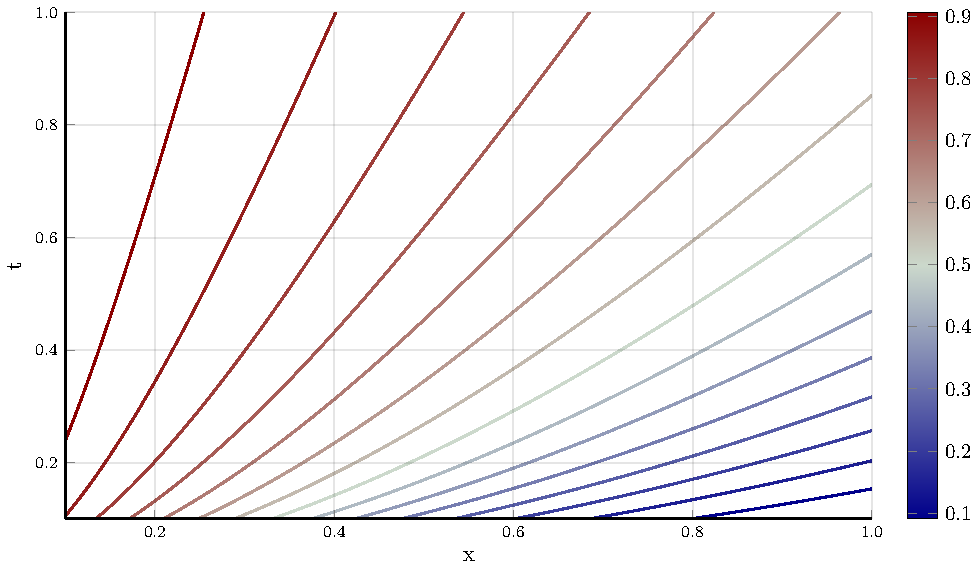
\includegraphics[width=\columnwidth]{./figures/advdif}}
\caption{Unsteady data from the 1D advection-diffusion equation}
\label{fig:advdif}
\end{center}
\vskip -0.2in
\end{figure}

To apply SIEO, the exact solution was sampled at 200 temporal points in the range $t = [0, 0.1]$ and between 10 and 200 spatial points. Then, additive white Gaussian noise at a level $\eta \in [0, 0.2]$ was added to the data such that the standard deviation of the noise is given by $\sigma = \eta \ {\rm std}(u)$. The grammar shown in \cref{fig:advdifgrammar} was used for the expression optimization routine and was limited to a tree depth of 3. The adjusted $R^2$ loss function was used with the parameter $\alpha = 0.5$ and the solution was denoised before and after the numerical differentiation using total variation filtering \cite{rudin1992nonlinear}.

\begin{figure}
    \vskip -0.2in
    \centering
    \begin{equation*}
    \begin{split}
    \mathbb{R} &\mapsto u \\
    \mathbb{R} &\mapsto \frac{d\mathbb{R}}{dx} \\
    \mathbb{R} &\mapsto \mathbb{R} \times \mathbb{R} \\
    \mathbb{R} &\mapsto \mathbb{R} / \mathbb{R}
    \end{split}
    \end{equation*}
    \vskip -0.15in
    \caption{Grammar used for the advection-diffusion equation}
    \label{fig:advdifgrammar}
    \vskip -.15in
\end{figure}

The results of six test cases are shown in \cref{tab:advdifresults}. After the trial number, the first two columns show the number of spatial sample points used and the noise level, respectively. The last two columns show the percent error in the model parameters, $v$ and $D$ when compared to their exact values. In all six test cases, SIEO determined the correct form of the governing equation. When the noise is 1--5\% and the number of sample points is 35 or larger, the error in the parameters remains small. In the two most challenging test cases (trials 3 and 6), the fit parameters $v$ and $D$ show high levels of error but the correct form of the equation was still discovered accurately which demonstrates the robustness of SIEO to find an accurate and generalizable model with large amounts of noise or limited data.

\begin{table}[t]
\caption{Error in solution parameters for different noise levels and spatial resolutions}
\label{tab:advdifresults}
\vskip 0.15in
\begin{center}
\begin{small}
\begin{sc}
\begin{tabular}{lccccr}
\toprule
 & Sample &  & Error & Error\\
Trial & Points & Noise & in $v$ & in $D$\\
\midrule
1 & 200 & 1\%  & 0.78 \% & 1.54 \% \\
2 & 200 & 5\%  & 5.64 \% & 2.84 \% \\
3 & 200 & 20\%  & 30.12 \% & 6.60 \% \\
4 & 100 & 0\%  & 0.84 \% & 0.29 \% \\
5 & 35 & 0\%  & 6.38 \% & 2.21 \% \\
6 & 10 & 0\%  & 49.08 \% & 19.02 \% \\
\bottomrule
\end{tabular}
\end{sc}
\end{small}
\end{center}
\vskip -0.1in
\end{table}


\subsection{Navier-Stokes Equations}
The second test system is the incompressible 2D Navier-Stokes equations which describe the motion of a viscous fluid. The Navier-Stokes equations are given by
\begin{align}
  \frac{\partial u}{\partial x} + \frac{\partial v }{\partial y} &= 0 \\
  \frac{\partial u }{\partial t} + u \frac{\partial u }{\partial x} + v \frac{\partial u }{\partial y} &= - \frac{1}{\rho} \frac{\partial p}{\partial x} + \frac{\mu}{\rho}\left( \frac{\partial^2 u}{\partial x^2} + \frac{\partial^2 u}{\partial y^2} \right) \\
\frac{\partial v }{\partial t} + u \frac{\partial v }{\partial x} + v \frac{\partial v }{\partial y} &= - \frac{1}{\rho} \frac{\partial p}{\partial y} + \frac{\mu}{\rho}\left( \frac{\partial^2 v}{\partial x^2} + \frac{\partial^2 v}{\partial y^2} \right)
\end{align}

where $\rho$ is the fluid density, $(u, v)$ is the fluid velocity, $p$ is the pressure, and $\mu$ is the viscosity. The first equation represents the conservation of mass and the next two equations represent conservation of momentum in the $x$ and $y$ directions, respectively. These equations are nonlinear, have multiple dimensions ($x$ and $y$) and multiple state variables ($u$, $v$, and $p$), which makes them a challenging model system to identify.

Synthetic data was collected from the simulation of vortex shedding behind a circular cylinder at a Reynold's number of 50. The simulation was performed using PyFR \cite{witherden2014pyfr} and 10 snapshots were taken with a timestep of $dt = 0.001$, $M = 0.2$ and $\rho \approx 1$ (with a very small amount of compressibility in the solution). A single frame of the simulation is shown in \cref{fig:ns_data}, with $u$, $v$, and $p$ on separate plots. The grammar in \cref{fig:nsgrammar} was used to produce features up to a depth of 3, yielding 363 features and $2^{363}$ mappings to be searched.

\begin{figure}
  \vskip 0.2in
    \subfloat[$x$-velocity]{\label{xvelocity}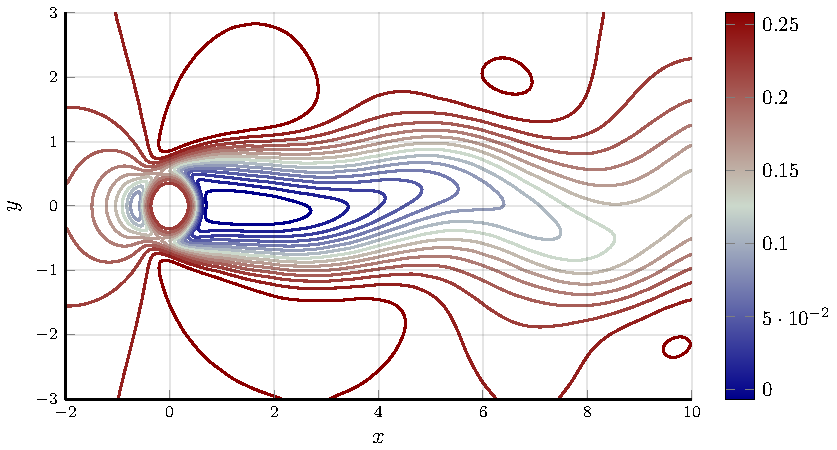
\includegraphics[width=0.977\columnwidth]{./figures/xvel}} \\
    \subfloat[$y$-velocity]{\label{yvelocity}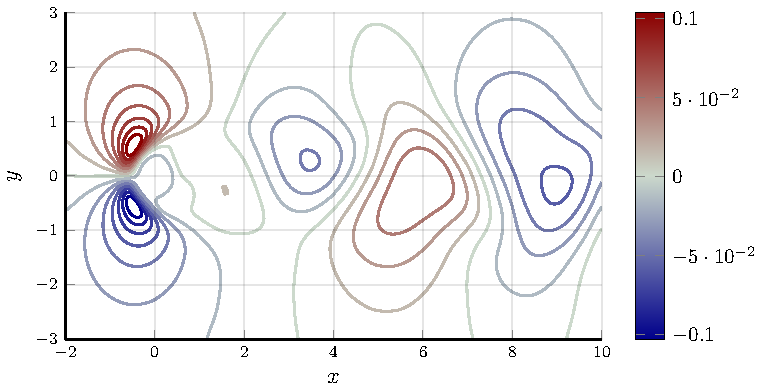
\includegraphics[width=\columnwidth]{./figures/yvel}} \\
    \subfloat[pressure]{\label{pressure}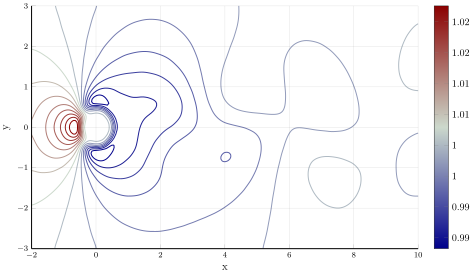
\includegraphics[width=0.94\columnwidth]{./figures/pressure}}
    \caption{One snapshot of vortex-shedding behind a circular cylinder}
    \label{fig:ns_data}
    \vskip -0.2in
\end{figure}

\begin{figure}
\vskip -0.15in
\centering
    \begin{equation*}
        \begin{split}
          \mathbb{R} &\mapsto u \quad | \quad v \quad | \quad p \\
          \mathbb{R} &\mapsto \frac{d\mathbb{R}}{dx} \quad \left| \quad \frac{d\mathbb{R}}{dy} \right. \\
          \mathbb{R} &\mapsto \mathbb{R} \times \mathbb{R}
        \end{split}
    \end{equation*}
    \vskip -0.15in
    \caption{Grammar used for the Navier-Stokes equations}
    \label{fig:nsgrammar}
    \vskip -.15in
\end{figure}

SIEO was performed on the the vortex shedding data with the adjusted $R^2$ loss function and $\alpha = 0.2 $ and it found ~\cref{eqn:xmom,eqn:ymom} to explain the unsteady Navier-Stokes data
\begin{align}
\label{eqn:xmom}
    \frac{\partial u}{\partial t} &= {\theta_x}_1 \frac{\partial  (u v)}{\partial y} + {\theta_x}_2 v \frac{\partial u}{\partial y} + {\theta_x}_3 \frac{\partial p}{\partial y} + {\theta_x}_4 \frac{\partial^2 u}{\partial y^2} \\
\label{eqn:ymom}
    \frac{\partial v}{\partial t} &= {\theta_y}_1 u \frac{\partial v}{\partial x} + {\theta_y}_2 v \frac{\partial v}{\partial y} + {\theta_y}_3 \frac{\partial p}{\partial y}
\end{align}
The first equation requires the substitution $\partial v /\partial y = - \partial u / \partial x $ (from the continuity equation) to transform it to the more well-known form of the $x$-momentum equation. Note also the absence of the viscous terms $\partial^2 u / \partial x^2$, $\partial^2 v / \partial x^2$, and $\partial^2 v / \partial y^2$. These terms are not included because in this particular fluid flow they are much smaller in magnitude than the other terms in the governing equation. This shows that for SIEO to identify a process, that process must have a sufficiently large signal in the data collected. 

The ratios of the model coefficients were compared to determine the error in the model parameters. The results are shown in \cref{tab:ns_data}. In general, the model parameter error is very small and the discovered equations could be used for prediction or control of other similar types of flow fields (i.e. those that do not have significant contributions from the three omitted viscous terms).

\begin{table}[t]
\caption{Error in Navier-Stokes Coefficients}
\label{tab:ns_data}
\vskip 0.15in
\begin{center}
\begin{small}
\begin{sc}
\begin{tabular}{lccccr}
\toprule
Parameter & Error \\
\midrule
${\theta_x}_2 / {\theta_x}_1 $ & 2.87 \% \\
${\theta_x}_3 / {\theta_x}_1 $ & 1.00 \% \\
${\theta_x}_4 / {\theta_x}_1 $ & 2.53 \% \\
${\theta_y}_2 / {\theta_x}_1 $ & 8.47 \% \\
${\theta_y}_3 / {\theta_x}_1 $ & 0.92 \% \\
\bottomrule
\end{tabular}
\end{sc}
\end{small}
\end{center}
\vskip -0.1in
\end{table}

\subsection{Exact Koopman Eigenfunction Discovery}
\label{exactdiscovery}
A simple nonlinear ODE with finite-dimensional Koopman eigenfunctions that are easily found is given by \citet{kutz2016dynamic} as
\begin{align}
 \label{simplekoopman1}
 \frac{dx}{dt} &= \mu x \\
 \label{simplekoopman2}
 \frac{dy}{dt} &= \lambda(y - x^2)
 \end{align}
 
The state-space transformation
\begin{equation}
    \label{eqn:exacttransform}
\begin{bmatrix}
x\\
y
\end{bmatrix} \mapsto \begin{bmatrix}
x \\
y \\
x^2
\end{bmatrix}
\end{equation}
linearizes~\cref{simplekoopman2,simplekoopman1} to
\begin{equation}
    \label{eqn:koopmanop}
\frac{d}{dt} \begin{bmatrix}
x \\
y \\
x^2
\end{bmatrix} = \begin{bmatrix}
\mu & 0 & 0 \\
0 & \lambda & -\lambda \\
0 & 0 & 2 \mu
\end{bmatrix} \begin{bmatrix}
x \\
y \\
x^2
\end{bmatrix}
\end{equation}

To test the discovery of exact Koopman operators, data from the system (\cref{simplekoopman1,simplekoopman2}) was collected for $\lambda = \mu = 1$ with many initial conditions. The initial data is stored in an vector $\vec{x}^0$, then the solution is integrated forward one timestep and the result is stored in an output vector $\vec{x}^1$. SIEO was then applied with the average normalized sum of squares loss function $\ell_k$. The goal was to find a state-inclusive Koopman operator, so the loss function was modified to penalize the absence of the primary state variables $x$ and $y$. The function-rich grammar in \cref{fig:odegrammar} was used as input (exchanging ($\theta$, $\omega$) for ($x$, $y$)). The correct Koopman transformation was discovered (\cref{eqn:exacttransform}) and the Koopman operator (\cref{eqn:koopmanop}) was recovered to within machine precision after a few seconds of computation running on a single thread of an Intel Core i5 processor.


\subsection{Approximate Koopman Eigenfunction Discovery of Nonlinear Pendulum}
One of the simplest nonlinear ODEs without a known Koopman operator is a simple pendulum swinging at large angles. The equation of motion a pendulum (with parameters normalized to 1) is given by
\begin{equation}
\frac{d^2 \theta}{d t^2} + \sin \theta = 0 \end{equation}
This equation can be converted to a system of nonlinear first-order ODEs given by
\begin{align}
\frac{d\theta}{dt} &= \omega \\
\frac{d\omega}{dt} &= -\sin \theta
\end{align}


\begin{figure}
\vskip -0.15in
\centering
\begin{equation*}
    \begin{split}
        \mathbb{R} &\mapsto \theta \quad | \quad \omega \\
        \mathbb{R} &\mapsto \mathbb{R} \times \mathbb{R} \\
        \mathbb{R} &\mapsto \sin (\mathbb{G} \times \mathbb{R}) \quad | \quad \sin (\mathbb{G} \times \mathbb{R} + \mathbb{G}) \\
        \mathbb{R} &\mapsto {\rm exp}(\mathbb{G} \times \mathbb{R}) \\
        \mathbb{R} &\mapsto 1 / (1 + {\rm exp}(-\mathbb{G} \times \mathbb{R})) \\
        \mathbb{R} &\mapsto {\rm exp}(-(\mathbb{R}-\mathbb{G})^2/\mathbb{G}) \\
        \mathbb{R} &\mapsto {\rm imag}(\mathbb{R}^\mathbb{G}) \\
        \mathbb{R} &\mapsto {\rm real}(\mathbb{R}^\mathbb{G}) \\
        \mathbb{G} &\mapsto -\mathbb{G} \quad | \quad \mathbb{G}+\mathbb{G} \quad | \quad \mathbb{G}/\mathbb{G} \\
        \mathbb{G} &\mapsto {\rm logspace(-5, 2, 20)}
    \end{split}
\end{equation*}
    \vskip -0.15in
    \caption{Grammar used for both nonlinear ODEs}
    \label{fig:odegrammar}
    \vskip -.15in
\end{figure}

In order to generate training data, the system was integrated forward in time from a starting position $(\theta_0, \omega_0) = (\pi/2, 0)$ until $T=10$. The Koopman operator was approximated by SIEO using the average sum of squares loss function with the same state-inclusive penalty described in \cref{exactdiscovery}. The function-rich grammar shown in \cref{fig:odegrammar} was used as the input. 

The resulting Koopman operator approximation with $24$ features was then compared to a linearized version of the equation with only the primary state variables. Both linear models were initialized at $(\theta_0, \omega_0) = (\pi/2, 0)$ and were allowed to evolve forward in time past the training period. The error between the linear model and the exact solution for each model is shown in \cref{fig:pendulum}.

The figure shows that the linear model with more nonlinear features has significantly lower average error than the linear model with only the two state variables. Additionally, the error increases more slowly for the Koopman approximation. This shows that it is possible to improve linearizations of nonlinear model by using expression optimization to approximate the Koopman eigenfunctions of the system.

\begin{figure}
\vskip 0.2in
\begin{center}
\centerline{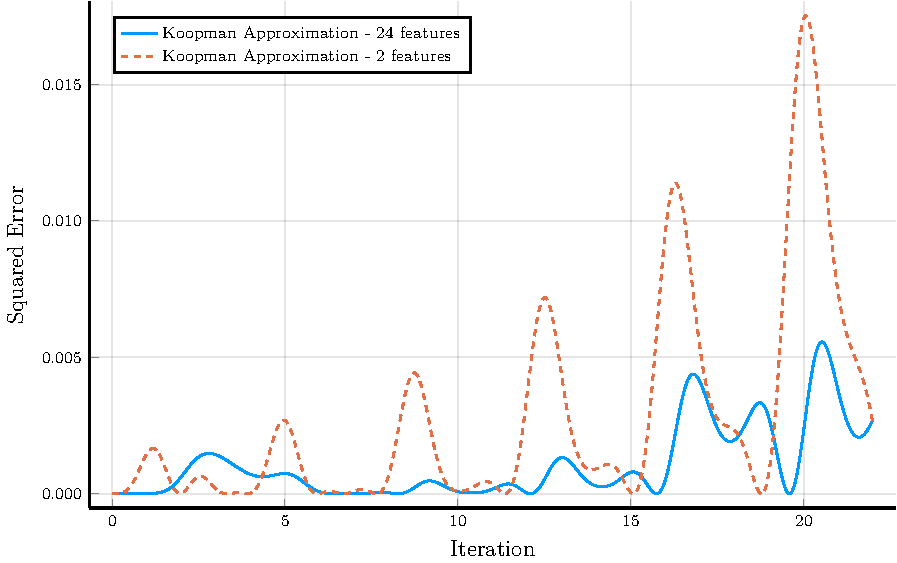
\includegraphics[width=\columnwidth]{./figures/pendulum}}
\caption{Error in the nonlinear pendulum for the simplest linear model and the linear model with 24 features}
\label{fig:pendulum}
\end{center}
\vskip -0.2in
\end{figure}

\section{Conclusions and Future work}
\label{conclusion}

From the previous experiments, we conclude that the use of context-free grammars and expression optimization is an effective way of generating mappings that describe observed data. The system is robust to noise and can operate on small amounts of data. Additionally, it is robust to multiple dimensions and variables in the state space. Lastly, it has been demonstrated that expression optimization has the potential to discover exact and approximate analytical Koopman eigenfunctions for the linearization of nonlinear systems. 

Further work on this topic will focus on expanding the utility of SIEO by 
\begin{itemize}
\item Including free-parameter optimization into the selection of expressions.
\item Investigating which grammars perform best for equation discovery and Koopman eigenfunction approximation.
\item Finding the Koopman eigenfunction approximations for larger dynamical systems and using the resulting models for control.

\end{itemize}



% Acknowledgements should only appear in the accepted version.
% \section*{Acknowledgements}

% In the unusual situation where you want a paper to appear in the
% references without citing it in the main text, use \nocite

\bibliography{ICML_SIEO}
\bibliographystyle{icml2019}


\end{document}


% This document was modified from the file originally made available by
% Pat Langley and Andrea Danyluk for ICML-2K. This version was created
% by Iain Murray in 2018, and modified by Alexandre Bouchard in
% 2019. Previous contributors include Dan Roy, Lise Getoor and Tobias
% Scheffer, which was slightly modified from the 2010 version by
% Thorsten Joachims & Johannes Fuernkranz, slightly modified from the
% 2009 version by Kiri Wagstaff and Sam Roweis's 2008 version, which is
% slightly modified from Prasad Tadepalli's 2007 version which is a
% lightly changed version of the previous year's version by Andrew
% Moore, which was in turn edited from those of Kristian Kersting and
% Codrina Lauth. Alex Smola contributed to the algorithmic style files.
